\documentclass[12pt]{article}

\usepackage{graphicx}
\usepackage{float}
\usepackage{amsmath}
\usepackage{amssymb}
\usepackage{graphicx}
\usepackage[utf8]{inputenc}
\usepackage[spanish]{babel}
\usepackage{geometry}
\geometry{left=2cm,right=2cm,top=2cm,bottom=2cm}
\usepackage{listings}
\lstset{basicstyle=\ttfamily,
  showstringspaces=false,
  commentstyle=\color{red},
  keywordstyle=\color{blue}
}


\title{%
  OpenGL Shading Language\\
  \large Tarea 07 \\
    \Large Computación Gráfica\\
     \large UNAM 2022-2}
\author{Gibran Zazueta Cruz \\
\small 19/mayo/2022}
\date{}

\begin{document}
\maketitle

\section{Introducción}

En el siguiente trabajo se realiza el renderizado de un objeto sobre una ventana utilizando OpenGL y OpenGL Shader language (GLSL).

Para crear la ventana se utiliza la biblioteca de QT y para importar objetos wavefront OBJ la biblioteca de assimp. El objeto elegido para renderizar es el conejo de stanford

La versión de OpenGL utilizada es la 4.5

\subsection{GLSL}
GLSL e un lenguaje de alto nivel, con syntax basado en \textit{C}, que permite 'interferir' en el pipeline gráfico de OpenGL.
Algunos tipos de shaders que permite implementar OpenGL son Vertex, Fragment, Tesselation y Geometry. EStos influyen en diferentes partes del pipeline.
En este trabajo se implementa un vertex y fragment shader.

\subsection{Escena y materiales}

El objeto cuentan con 2 posibles materiales a seleccionar, estos se definen dentro del código como:

\textbf{Material 1}
\begin{itemize}
\item Ambiental = {0.0, 0.0, 0.0, 1.0},
\item Difusa = {0.50, 0.50, 0.50, 1.0},
\item Especular {0.70, 0.70, 0.70, 1.0} 
\item $\rho$ = 32.0.
\end{itemize}


\textbf{Material 2}
\begin{itemize}
\item Ambiental = {0.23125, 0.23125, 0.23125, 1.0},
\item Difusa = {0.2775, 0.2775, 0.2775, 1.0},
\item Especular {0.773911, 0.773911, 0.773911, 1.0}
\item $\rho$ = 89.6.
\end{itemize}


La escena a renderizar cuenta con 2 luces (blanca y azul) y 3 cámaras. Las cámaras se definen con un FOV de $45º$



\section{Estructura del código}

Para almacenar la información del objeto se define la clase \textit{CubeObject} y la  función \textit{importFile()}, definida en \textit{functions.cpp}.

Esta función se llama desde \textit{mainwindow.cpp}. La función recibe el path del archivo (como una cadena) y apuntadores al contenedor de vertices, indices de caras, normales y coordenadas de textura del objeto cubeObject, que es el objeto  a renderizar en la escena. Dentro de esta función se utiliza la bilbioteca de assimp para importar el objeto.
\\
\\
En la función \textit{initializeGL()} de \textit{mainwindow} se declara la variable \textit{program} de la clase \textit{QOpenGLShaderProgram()}. Esta clase de QT maneja el compilado y linking de shaders escritos es GLSL.
El código es agregado desde los archivos fuente $'shader.vert'$ y $'shader.frag'$.
\\
\\
En la función \textit{paintGL} se utilizan matrices del tipo \textit{QMatrix4x4} para contener las matrices de proyección, view y model de la cámara y objeto. Estas matrices se pasan al Vertex shader (como uniform mat4) para realizar la proyección en perspectiva.
Por otro lado al Fragment shader se asignan los valores relacionados con la posición y color de las luces y la información del material actual del objeto.
\\
\\
\textbf{\textit{Fragment Shader}}
\\
Se implementa sombreado de phong utilizando las ecuaciones de luz difusa y especular.
El shader recibe del vertex shader los valores interpolados de las normales y la posición de cada fragmento. También recibe del programa la información de las luces y del material. Las ecuaciones se implementan para cada una de las 2 luces de la escena.

\section{Ejecutar el programa}
En la carpeta de build se puede ejecutar el programa con el archivo GLSLRendering-Run. Desde la consola de comandos de linux:

\begin{lstlisting}[language=bash,title={bash}]
./GLSLRendering-Run
\end{lstlisting}


En la carpeta principal está el código fuente. Para generar el ejecutable primero se genera el Makefile con

\begin{lstlisting}[language=bash,title={bash}]
 qmake GLSLRendering.pro
\end{lstlisting}

Después se construye el proyecto con \textit{make}



\section{Instrucciones de uso}


Para cambiar entre las camaras se utilizan las teclas de los numeros
\begin{itemize}
\item "1". Cambia a la cámara 1
\item "2". Cambia a la cámara 2
\item "3". Cambia a la cámara 3
\item "4". Cambia a la cámara 4

\end{itemize}


Para encender y apagar la luz azul se presiona la tecla \textbf{\textit{L}}. La luz inicia encendida.

Para activar y desactivar el sombreado de Phong se presiona la tecla \textbf{\textit{P}}. El sombreado inicia activo

Para cambiar entre materiales se utiliza la tecla \textbf{\textit{8}} para el material 1 y la tecla \textbf{\textit{9}} para el material 2.




\section{Programa en ejecución}

\begin{figure}[H]
\centering
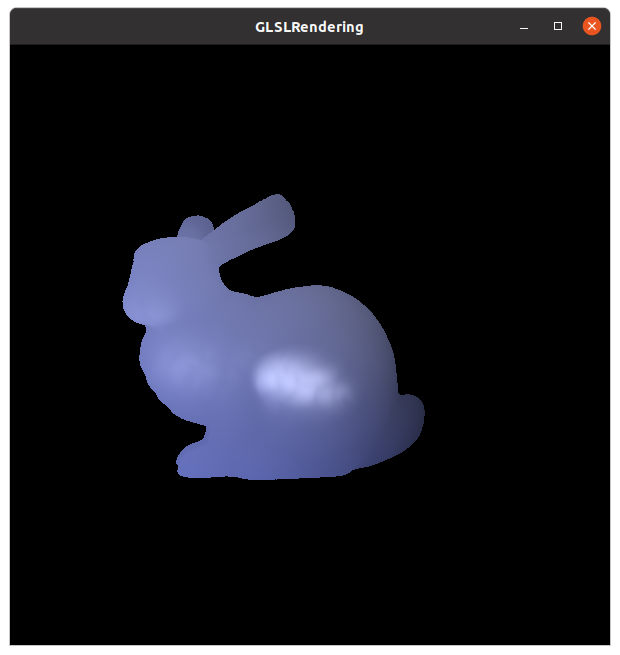
\includegraphics[scale=0.3]{images/ej1.png}
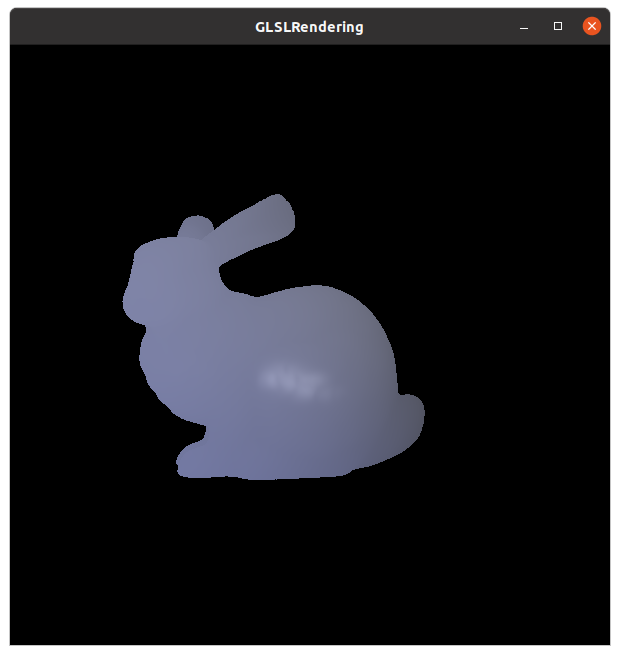
\includegraphics[scale=0.3]{images/ej2.png}
\caption{Renderizado cámara 1, materiales 1 y 2}
\end{figure}

\begin{figure}[H]
\centering
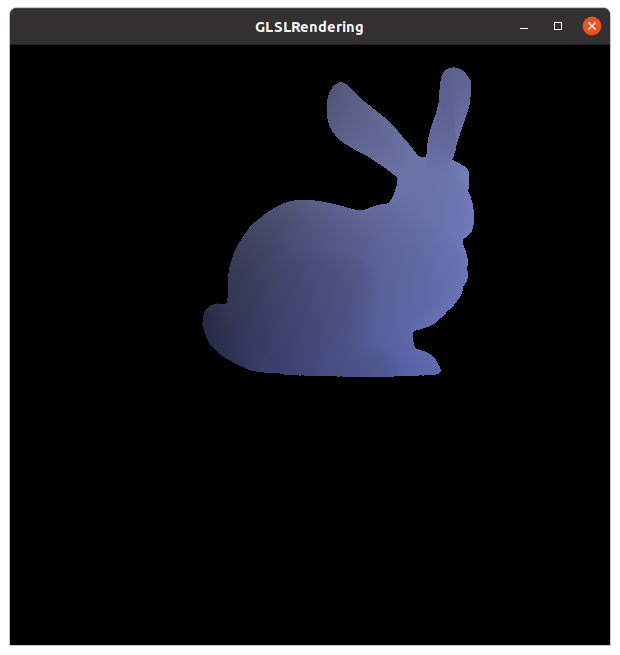
\includegraphics[scale=0.3]{images/ej3.png}
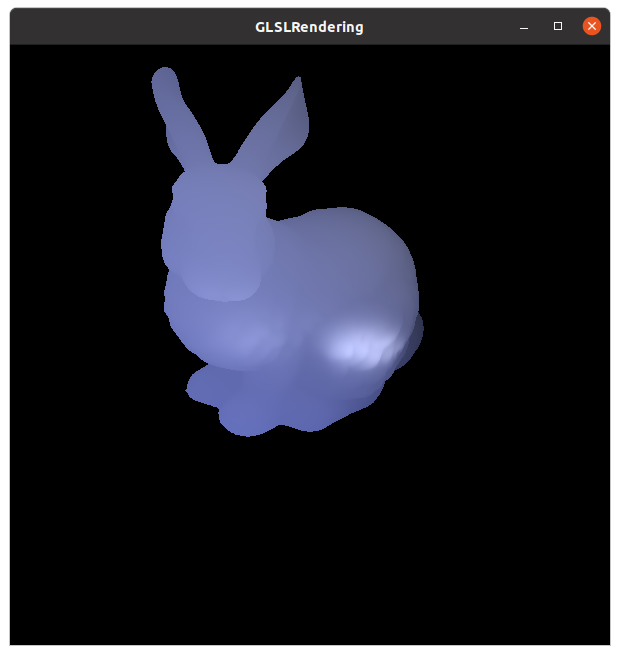
\includegraphics[scale=0.3]{images/ej4.png}
\caption{Renderizado cámara 2, 3 . Material 1}
\end{figure}


%\begin{thebibliography}{99}


%\end{thebibliography}


\end{document}
